\documentclass[10pt, a4paper]{ctexart}
\usepackage[margin=1in]{geometry}
\usepackage{bm}
\usepackage{amsmath}
\usepackage{graphicx}
\usepackage{float}
\usepackage{listings}

\begin{document}
\title{Assignment 1}
\date{}
\author{}
\maketitle

\section{Softmax}
{\bf{(a)}} Proof:
\begin{align*}
    {\rm{softmax}}({\bm{x}}+c)_i &= \frac{e^{x_i+c}}{\sum_je^{x_j+c}}\\
    &=\frac{e^{x_i}e^c}{\sum_j\big(e^{x_j}e^c\big)}\\
    &=\frac{e^{x_i}}{\sum_je^{x_j}}\\
    &={\rm{softmax}}({\bm{x}})_i
\end{align*}\par
{\bf{(b)}} See file q1\_softmax.py

\section{Neural Network Basic}
{\bf{(a)}} We have:
\begin{align*}
    \sigma(x)'&=\frac{1}{(1+e^{-x})^2}e^{-x}\\
    &=\frac{1}{1+e^{-x}}\frac{e^{-x}}{1+e^{-x}}\\
    &=\sigma(x)\big(1-\sigma(x)\big)
\end{align*}\par
{\bf{(b)}} Because $\bm y$ is a one-hot label, we can assume that all elements in it is zero, except that the kth element is one. Therefore, by using the chain rule, we have:
\begin{align*}
    \frac{\partial CE}{\partial {\bm \theta_i}}&=\frac{\partial CE}{\partial {\bm {{\hat y}}}}\frac{\partial {\bm{\hat y}}}{\partial {\bm \theta_i}}\\
    &=-\frac{1}{{\bm {\hat{y}}_k}} \frac{\partial {\bm{\hat y}}}{\partial {\bm \theta_i}}\\
\end{align*}
For $i=k$, we have:
\begin{align*}
    \frac{\partial {\bm{\hat y}}}{\partial {\bm \theta_k}}=-\frac{e^{x_k}\sum_{j\ne k}e^{x_j}}{(\sum_j{e^{x_j}})^2}
\end{align*}
For $i\ne k$, we have:
\begin{align*}
    \frac{\partial {\bm{\hat y}}}{\partial {\bm \theta_i}}=\frac{e^{x_k}e^{x_i}}{(\sum_j{e^{x_j}})^2}
\end{align*}
Therefore, we have:
\begin{equation*}
    \frac{\partial CE}{\partial {\bm \theta}}={\bm{\hat{y}}}-{\bm y}
\end{equation*}\par
{\bf{(c)}} By using the result from the above question, we know that:
\begin{align*}
    \frac{\partial CE}{\partial {\bm h}}=({\bm{\hat{y}}}-{\bm y}){\bm W_2}^T
\end{align*}
Let ${\bm{O_1}}={\bm x}{\bm W_1}+{\bm b_1}$, and by using the result of question (a), we have:
\begin{align*}
    \frac{\partial CE}{\partial {\bm O_1}}=({\bm{\hat{y}}}-{\bm y}){\bm W_2}^T*{\bm h}(1-{\bm h})
\end{align*}
Therefore, we have:
\begin{align*}
    \frac{\partial CE}{\partial {\bm x}}=\Big(({\bm{\hat{y}}}-{\bm y}){\bm W_2}^T*{\bm h}(1-{\bm h})\Big)W_1^T
\end{align*}\par
{\bf{(d)}} The dimension of $W_1$ is $D_x\times H$ and the dimension of $W_2$ is $H\times D_y$. Therefore, the total number of parameters are $D_x\times H+H\times D_y+H+D_y$\par
{\bf{{(e)}}} See file q2\_sigmoid.py\par
{\bf{{(f)}}} See file q2\_gradcheck.py\par
{\bf{(g)}} See file q2\_neural.py

\section{word2vec}
{\bf{(a)}} Let ${\bm U}=[{\bm \mu}_1, {\bm \mu}_2,\dots, {\bm \mu}_v]$ where each column represents an "output" word vector for some word in the vocabulary. The gradient of loss with respect to ${\bm v}_c$ is given by:
\begin{align*}
    \frac{\partial CE}{\partial {\bm v}_c}&=-\frac{1}{\hat{y}_o}\frac{\partial \hat{y}_o}{\partial{\bm v}_c}\\
    &=\frac{1}{\hat{y}_o}\frac{\bigg(\sum_{w=1}^V\big(({\bm \mu}_w-{\bm \mu}_o)\exp({\bm \mu}_w^T{\bm v}_c)\big)\bigg)\exp({\bm \mu}_o^T{\bm v}_c)}{\bigg(\sum_{w=1}^V\exp({\bm \mu}_w^T{\bm v}_c)\bigg)^2}\\
    &=\frac{\sum_{w=1}^V\big(({\bm \mu}_w-{\bm \mu}_o)\exp({\bm \mu}_w^T{\bm v}_c)\big)}{\sum_{w=1}^V\exp({\bm \mu}_w^T{\bm v}_c)}
\end{align*}\par
{\bf{(b)}}For ${\bm \mu}_k$ where $k\ne o$, we have:
\begin{align*}
    \frac{\partial CE}{\partial {\bm \mu}_k}&=\frac{1}{\hat{y}_o}\frac{\exp({\bm \mu}_o^T{\bm v}_c)\exp({\bm \mu}_k^T{\bm v}_c){\bm v}_c}{\bigg(\sum_{w=1}^V\exp({\bm \mu}_w^T{\bm v}_c)\bigg)^2}\\
    &=\frac{\exp({\bm \mu}_k^T{\bm v}_c){\bm v}_c}{\sum_{w=1}^V\exp({\bm \mu}_w^T{\bm v}_c)}
\end{align*}\par
For ${\bm \mu}_o$, we have:
\begin{align*}
    \frac{\partial CE}{\partial {\bm \mu}_o}&=-\frac{1}{\hat{y}_o}\frac{{\bm v}_c\exp({\bm \mu}_o^T{\bm v}_c)\sum_{w=1,~w\ne o}^V\exp({\bm \mu}_w^T{\bm v}_c)}{\bigg(\sum_{w=1}^V\exp({\bm \mu}_w^T{\bm v}_c)\bigg)^2}\\
    &=-\frac{{\bm v}_c\sum_{w=1,~w\ne o}^V\exp({\bm \mu}_w^T{\bm v}_c)}{\sum_{w=1}^V\exp({\bm \mu}_w^T{\bm v}_c)}
\end{align*}\par
{\bf{(c)}} The gradient of negative sampling loss with respect to ${\bm v}_c$ is given by:
\begin{align*}
    \frac{\partial J_{NS}}{\partial {\bm v}_c} = (\sigma({\bm \mu}_o^T{\bm v}_c)-1){\bm \mu}_0-\sum_{k=1}^K\bigg((\sigma(-{\bm \mu}_k^T{\bm v}_c)-1){\bm \mu}_k\bigg)
\end{align*}\par
The gradient of loss with respect to ${\bm \mu}_k$ where $k\ne o$ is given by:
\begin{align*}
    \frac{\partial J_{NS}}{\partial {\bm \mu}_k}=(1-\sigma(-{\bm \mu}_k^T{\bm v}_c)){\bm v}_c
\end{align*}
And the gradient of loss with respect to ${\bm \mu}_o$ is given by:
\begin{align*}
    \frac{\partial J_{NS}}{\partial {\bm \mu}_o}=(\sigma({\bm \mu}_o^T{\bm v}_c)-1){\bm v}_c
\end{align*}\par
This cost function is much more efficient compared to softmax loss because in softmax loss we have to iterate through all words in vocabulary to calculate the inner product with the word vector of the center word, while in the negative sampling loss function, we just have to pick k random words and calculate the inner product, which gives us approximately $\frac{V-K}{V}$ speed up.\par
{\bf{(d)}} In Skip-Gram, the gradient for word vector $w_{i}$ where $t-m \le i \le t+m$ and $i\ne t$ is given by:
\begin{align*}
    \frac{\partial J_{SG}}{\partial w_i}=\sum_{-m\le j\le m,j\ne 0}\frac{\partial F(w_j, {\bm v}_c)}{\partial w_i}
\end{align*}
And the gradient for center word ${\bm v}_c$ is given by:
\begin{align*}
    \frac{\partial J_{SG}}{\partial {\bm v}_c}=\sum_{-m\le j\le m,j\ne 0}\frac{\partial F(w_j,{\bm v}_c)}{\partial {\bm v}_c}
\end{align*}\par
For CBOW, the gradient for $w_t$ is given by:
\begin{align*}
    \frac{\partial J_{CBOW}}{\partial w_t}=\frac{\partial F(w_t, {\bm{\hat{v}}})}{\partial w_t}
\end{align*}
And the gradient for ${\bm v}_i$ where $t-m\le i\le t+m$ and $i\ne t$ is given by:
\begin{align*}
    \frac{\partial J_{CBOW}}{\partial {\bm v}_i}=\frac{\partial F(w_t, {\bm{\hat v}})}{\partial {\bm{\hat v}}}
\end{align*}\par
{\bf{(e)}} See file q3\_word2vec.py\par
{\bf{(f)}} See file q3\_sgd.py\par
{\bf{(g)}} The plot is:
\begin{figure}[H]
    \centering
    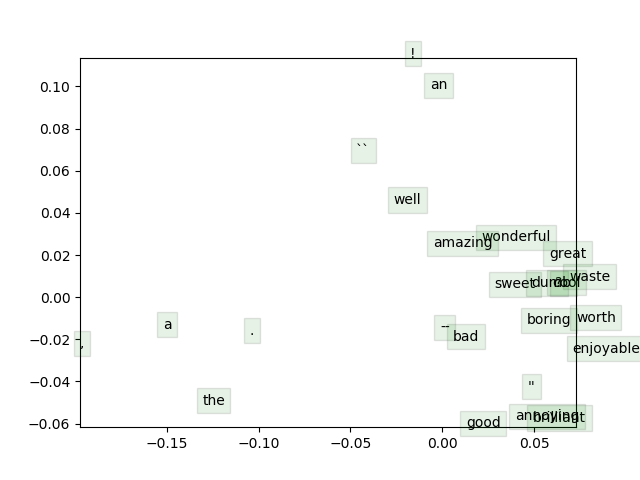
\includegraphics[width=0.7\linewidth]{../q3_word_vectors.png}
    \caption{Visualization of Word Vectors}
\end{figure}\par
As we can see from the plot, all adjective words are clustered together at the bottom right corner of the plot, while article words like "the" is on the other side of the plot.\par

\section{Sentiment Analysis}
{\bf{(a)}} See file q4\_sentiment.py\par
{\bf{(b)}} The reason why we want to introduce regularization when doing classification is to prevent overfitting.\par
{\bf{(c)}} See file q4\_sentiment.py. My code for {\emph{chooseBestModel}} is:
\begin{lstlisting}[language=python,numbers=left,numberstyle=\tiny,frame=single]
current_best_dev_acc = 0
for result in results:
    if result['dev'] > current_best_dev_acc:
        bestResult = result
        current_best_dev_acc = result['dev']
\end{lstlisting}\par
{\bf{(d)}} The best results are:
\begin{table}[H]
    \centering
    \begin{tabular}{c|c|c|c}
        \hline
        \hline
        &Train&Dev&Test\\
        \hline
        Our vectors&31.004\%&32.698\%&30.362\%\\
        Pretrained&39.934\%&36.512\%&37.014\%\\
        \hline
    \end{tabular}
\end{table}\par
The pretrained vectors are better because:
\begin{enumerate}
    \item These vectors are trained on a much larger data set.
    \item These vectors are trained for a much longer time.
    \item GloVe tends to work better than Skip-Gram and CBOW.
\end{enumerate}\par
{\bf{(e)}} The plot is:
\begin{figure}[H]
    \centering
    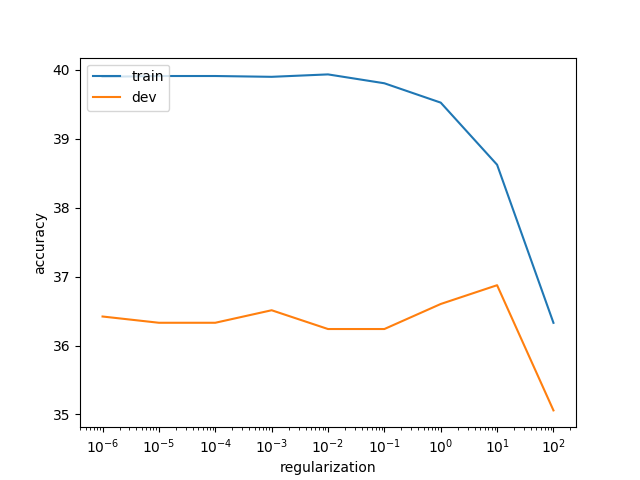
\includegraphics[width=0.7\linewidth]{../q4_reg_v_acc.png}
    \caption{Reg Value with respect to Dev and Train Acc}
\end{figure}\par
We can see from above that when regularization value is small, there is a huge gap between training accuracy and dev accuracy, meaning that we have encountered overfitting. As the regularization value increase, the gap becomes smaller, meaning that we have greatly reduced the overfitting. However, as the regularization value continues to increase, both the training accuracy and dev accuracy begin to fall, meaning that we may encounter underfitting.\par
{\bf{(f)}} The plot is:
\begin{figure}[H]
    \centering
    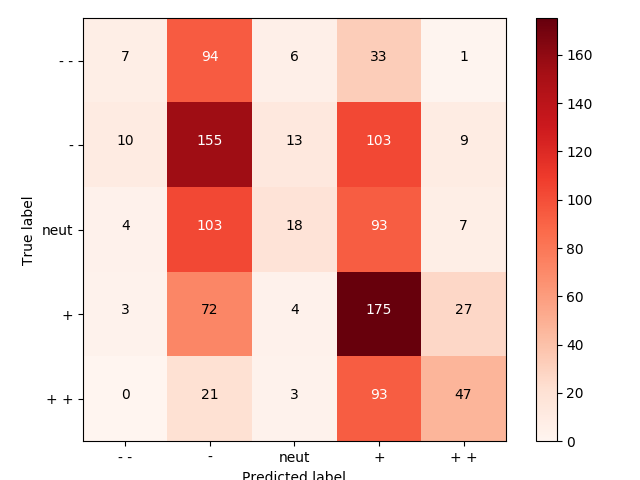
\includegraphics[width=0.7\linewidth]{../q4_dev_conf.png}
    \caption{Confusion Matrix on the Dev Set (with Pretrained Vectors)}
\end{figure}\par
It is easy to see from above that our model tends to predict a sentence more positive than it should be. Also, our model using the pretrained vectors works quite well that it usually only makes small mistakes (like predicting a positive sentence to be very positive) rather than big mistakes (like predicting a very negative sentence to be very positive).\par
{\bf{(g)}} For the following examples:
\begin{enumerate}
    \item Comment: like mike is a winner for kids, and no doubt a winner for lil bow wow, who can now add movies to the list of things he does well. Its ground truth is very positive (4), however, we predict it as negative (1). We will need feature "list of things he does well".
    \item Comment: this riveting world war ii moral suspense story deals with the shadow side of american culture: racial prejudice in its ugly and diverse forms. Its ground truth is negative (1), however we predict it as positive (3).
    \item Comment: a painfully funny ode to bad behavior. Its ground truth is positive (3), while we predict it as vert negative (0). This maybe is because our model sees words like "painfully" and "bad". The feature we need to classify it right is "ode".
\end{enumerate}
\end{document}